\section{Traditional Approaches to Graph Learning}
\subsection{Node-level statistics}
Prior to advent of deep learning on graphs, a large part of machine learning on graphs was directed towards extraction of statistics/features based on heuristic functions and domain knowledge from graphs, and passing this information to a machine learning classifier. Now, we look over common node-level statistics.
\begin{definition}[Node degree]
The degree $d_u$ of a node $u \in V$ is the number of edges incident to a node, and in terms of $\mathbf{A}$ for a simple graph
\begin{equation} \label{eq:degree}
	d_u = \sum_{v \in V} A_{uv}
\end{equation}
If our graph is directed or weighted, we can have the notion of in-degree and out-degree by summing over rows or columns in Equation (\ref{eq:degree}).
\end{definition}
\marginnote{\textit{Perron-Frobenius Theorem}: A real square matrix with positive entries has a unique largest real eigenvalue, and the corresponding eigenvector can be chosen to have strictly positive components.} \label{thm:perron}
\begin{definition}[Eigenvector Centrality]
The eigenvector centrality $e_u$ of a node $u \in V$ is defined by the recurrence relation
\begin{equation}
	e_u = \dfrac{1}{\lambda} \sum_{v\in V} A_{uv}e_v \; \forall \; u \in V
\end{equation}	
We can rewrite the above equation to notice that $\mathbf{A}\mathbf{e} = \lambda \mathbf{e}$ where $\mathbf{e}$ is the vector of node centralities.
\end{definition}
Note that, we want the centrality values to be positive, and by the \textbf{Perron-Frobenius Theorem}. 
In all, $\mathbf{e}$ is given by the eigenvector of the largest eigenvalue of $\mathbf{A}$. \marginnote{Note that the matrix $\mathbf{B}^{(n)}=\mathbf{A}^n$ has the elements such that $\mathbf{B}_{uv}^{(n)}$ denotes the number of $n-$length paths from $u \to v$.}
Now, since $\lambda$ is the leading eigenvalue, $e_u$ ranks the likelihood that a node is visited on a random-walk of infinite length on the graph as we can use power iteration method ($\mathbf{e^{(t)}} = \mathbf{A}\mathbf{e^{(t-1)}})$) to find $\mathbf{e}$. \\
By centrality, we can also measure how often a node lies on the shortest path between two nodes (\textit{betweeness centrality}), or average shortest path length between a node and all other nodes (\textit{closeness centrality}).
\begin{definition}[Clustering Coefficient]
The clustering coefficient \cite{small-world-dynamics} is given as
\begin{equation}
	c_u = \dfrac{|(v_1, v_2) \in E \; : \; v_1, v_2 \in \mathcal{N}(u)|}{{d_u \choose 2}}
\end{equation}	
It essentially measures the proportion of closed triangles in a node's local neighborhood.
\end{definition}
We can view clustering coefficient as the ratio between actual number of triangles and total possible number of triangles within a node's \textit{ego graph}: subgraph having the node, neighbors and all edges between nodes in its neighborhood.
\subsection{Graph Kernel Methods}
These methods are used for generating graph-level features for tasks such as graph classification.
\begin{definition}[Bag of Nodes]
Bag of nodes refers to aggregates of node-level statistics such as histograms based on clustering coefficients, and the use of such aggregates as graph-level features.
\end{definition}
Clearly bag of nodes misses global graph properties, and one way to improve it is to use iterative neighborhood aggregation.\\
    \begin{tcolorbox}[space to upper,
	skin=bicolor,
	colbacklower=black!75,
	collower=white,
	title={Weisfieler–Lehman Algorithm},
%	halign=center,
%	valign=center,
	nobeforeafter,
%	halign lower=flush right,
	bottom=0mm,
	height=6.4cm,
	width=4in
	]
	\begin{enumerate}
		\item Assign an initial label $\ell^{(0)}(v)$ to each node. A usual practice is to just assign the degree.
		\item Iteratively assign a new label by hashing the multiset of current labels within the neighborhood $$\ell^{(i)}(v) = \texttt{HASH}(\{\{\ell^{(i-1)}(u)\;\forall\;u \in \mathcal{N}(v)\}\})$$
		\item After running $K$ iterations of step-2, our label summarizes a $K$-hop neighborhood. Now use statistics of labels as features for the graphs.	
	\end{enumerate}
\end{tcolorbox}\\
\noindent The WL Kernel is computed by measuring the difference between the label sets of two graphs.
\begin{definition}[Graphlets]
Graphlets are small non-isomorphic induced subgraphs representing connected patterns in a network, and their frequency can be used to assess network structure.
\end{definition}
\begin{marginfigure}
	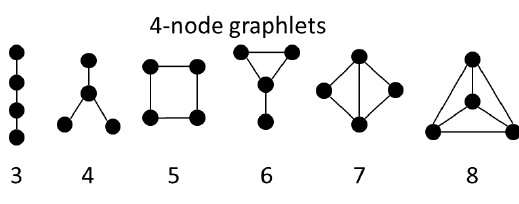
\includegraphics[width=\textwidth]{graphlets.png}
	\caption{Graphlets with 4 nodes}
	\label{fig:graphlets}
\end{marginfigure}
Graphlet kernels enumerate all graph structures of a possible size and count their occurrence in a graph. This is combinatorially difficult and an alternative is to use path-based methods which examine different kinds of paths in the graph. For example, the \textit{random-walk kernel} \cite{random-walk-kernel} involves running random walks all over the graph and then counting the occurrence of different degree sequences, while the \textit{shortest-path kernel} \cite{shortest-path-kernel} uses shortest paths between nodes instead of random-walks.

\subsection{Measures of Neighborhood Overlap}
Now we try to quantify the relation between nodes, which cannot be done using node-level or graph-level kernels. We denote $\mathbf{S} \in \mathbb{R}^{|V| \times |V|}$ as the similarity matrix summarizing the statistics. We commonly take the probability of an edge occurring proportional to the statistical measure, i.e $\mathbb{P}(A_{uv} = 1) \propto \mathbf{S}[u,v]$.
\begin{enumerate}
	\item \textit{Local overlap measures}
\begin{enumerate}
\item \textbf{Common Neighbors (CN)}: It is the simplest neighborhood overlap measure and counts the number of neighbors two nodes share.
\begin{equation}
	\mathbf{S}_{CN}[u, v] = |\mathcal{N}(u) \cap \mathcal{N}(v)|
\end{equation}	
We can extend the idea to local overlap measures defined over CN, denoted by the next three quantifiers.
\item \textbf{Sorensen index}: This normalizes the counts of common neighbours by the sum of node-degrees.
\begin{equation}
	\mathbf{S}_{Sorensen}[u, v] = \dfrac{2|\mathcal{N}(u) \cap \mathcal{N}(v)|}{d_u + d_v}
\end{equation}
\item \textbf{Salton index}: This normalizes using the product of degrees.
\begin{equation}
	\mathbf{S}_{Salton}[u, v] = \dfrac{2|\mathcal{N}(u) \cap \mathcal{N}(v)|}{\sqrt{d_ud_v}}
\end{equation}
\item \textbf{Jaccard index}: This is an IOU measure.
\begin{equation}
	\mathbf{S}_{Jaccard}[u, v] = \dfrac{|\mathcal{N}(u) \cap \mathcal{N}(v)|}{|\mathcal{N}(u) \cup \mathcal{N}(v)|}
\end{equation}
\item \textbf{Resource Allocation (RA)}: It places importance on the common neighbors by summing the inverse degrees, i.e
\begin{equation}
	\mathbf{S}_{RA}[u, v] = \sum_{w \in \mathcal{N}(u) \cap \mathcal{N}(v)} \dfrac{1}{d_w}
\end{equation}
\item \textbf{Adamic-Adar (AA)}: It is similar to RA, just utilizes inverse log of the degrees, i.e
\begin{equation}
	\mathbf{S}_{AA}[u, v] = \sum_{w \in \mathcal{N}(u) \cap \mathcal{N}(v)} \dfrac{1}{\log d_w}
\end{equation}
Both these measures infer that common neighbors with low degrees are more informative.
\end{enumerate}
\item \textit{Global overlap measures}
\begin{enumerate}
	\item \textbf{Katz Index}: We take a discounted count of number of paths of all lengths between a pair of nodes, i.e
	\begin{equation}
		\mathbf{S}_{Katz}[u, v] = \sum_{i=1}^\infty \beta^i A_{uv}^i = \Big((\mathbf{I} - \beta \mathbf{A})^{-1} - \mathbf{I}\Big)[u,v]
	\end{equation}
	Here $\beta \in \mathbb{R}^+$ is our discount, and a small $\beta < 1$ down-weights the importance of long-paths.
	\item \textbf{Leicht, Holme, and Newman Similarity}: The issue with Katz index is that it is biased towards high-degree nodes. To avoid that, we normalize the number of paths by its expectation, i.e $\frac{\mathbf{A}^i}{\mathbb{E}[\mathbf{A}^i]}$. The expectations can be computed by drawing a random graph with the same set of degrees as the graph under test, and obtain
	\begin{equation}
		\mathbb{E}[A_{uv}] = \dfrac{d_ud_v}{2|E|} \qquad \mathbb{E}[A_{uv}^2] = \dfrac{d_ud_v}{(2|E|)^2} \sum_{w \in V} d_w(d_w-1)
 	\end{equation}
 Calculation for $i > 2$ needs to be approximated, and to do so we utilize the fact mentioned earlier (\ref{thm:perron}) to notice that the growth is by a factor $\lambda$ for large $i$, and thus $\mathbb{E}[A_{uv}^i] = \dfrac{d_ud_v\lambda^{i-1}}{2|E|}$. Finally, the index is given as
 \begin{equation}
 	\mathbf{S}_{LHN}[u,v] = I_{uv} + \dfrac{2|E|}{d_ud_v}\sum_{i=0}^\infty \beta \lambda^{i-1}A_{uv}^i
 \end{equation}
\item \textbf{Random Walk Methods}: Take $\mathbf{D}$ to be a diagonal matrix with entries as the node degrees. Looking at the Personalized PageRank algorithm \cite{personalized-page-rank}, we define $\mathbf{P} = AD^{-1}$ and define vector $\mathbf{q}_u$ as the probability vector of visiting all nodes starting at node $u$. In a recursive fashion we incorporate the probability of restarting the random walk with probability $c$ and write $\mathbf{q}_u = c\mathbf{P}\mathbf{q}_u + (1-c)\mathbf{e}_u$ where $\mathbf{e}_u$ is a one-hot vector at node $u$. It's solution is
\begin{equation}
	\mathbf{q}_u = (1-c)(1-c\mathbf{P})^{-1}\mathbf{e}_u
\end{equation}
The similarity measure is
\begin{equation}
	\mathbf{S}_{RW}[u, v] = \mathbf{q}_u[v] + \mathbf{q}_v[u]
\end{equation}
\end{enumerate}
\end{enumerate}
\subsection{Graph Laplacians}
Laplacians are transformations of the adjacency matrix which have useful properties.
\begin{definition}[Unnormalized Laplacian]
	The unnormalized Laplacian is given by $\mathbf{L} = \mathbf{D}-\mathbf{A}$ and for simple graphs has the following properties:
	\begin{itemize}
		\item[$\diamond$] It is symmetric and positive semi-definite.
		\item[$\diamond$] For $\mathbf{x} \in \mathbb{R}^{|V|}$, \begin{equation}
			\mathbf{x}^T\mathbf{Lx} = \sum_{(u,v)\in E} (\mathbf{x}[u] - \mathbf{x}[v])^2
		\end{equation}
		\item[$\diamond$] The eigenvalues of $\mathbf{L}$ are non-negative.
		\item[$\diamond$] The geometric multiplicity of $\mathbf{L}$ denotes the number of connected components in the graphs.
	\end{itemize}
\end{definition}
We extend the definition to normalized Laplacians in two ways:
\begin{equation}
	\mathbf{L}_{sym} = \mathbf{D}^{-1/2}\mathbf{L}\mathbf{D}^{-1/2} \qquad \mathbf{L}_{RW} = \mathbf{D}^{-1}\mathbf{L}
\end{equation}
\subsection{Clustering using Laplacians}
We can extend property 4 of Laplacians to give optimal clustering within a fully-connected graph.
\begin{definition}[Graph Cut]
Let $U \subset V$ and let $\bar{U}$ be its complement. Given $K$ non-overlapping partitions of a graph $\{U_i\}_{i=1}^K$, we define the cut value as
\begin{equation}
	cut(U_1, \cdots, U_K) = \dfrac{1}{2}\sum_{k=1}^K|(u, v) \in E \; : \; u \in U_k, v \in \bar{U}_k|
\end{equation}
It essentially counts the number of edges crossing the boundary between partitions.
\end{definition}
\marginnote{\textbf{ 2-clustering over RatioCut:}\label{der:2-cluster} We solve \begin{equation*}
		\min_{U \in V} RatioCut(U, \bar{U})
	\end{equation*}
	Define $\mathbf{a} \in \mathbb{R}^{|V|}$ and $\xi = \sqrt{\frac{|\bar{U}|}{|U|}}$ such that $a_u = \xi$ if $u \in U$ else $a_u = -\frac{1}{\xi}$.
	With some calculation, we can show that 
	\[\mathbf{a}^T\mathbf{L}\mathbf{a} = |V|RatioCut(U, \bar{U})\]
	We can also show that
	\begin{enumerate}
		\item $\sum_{u \in V} a_u = 0 \Leftrightarrow \mathbf{a} \perp \mathbf{1}$
		\item $||a||^2 = |V|$
	\end{enumerate}
	Solving $\min_{U \in V}\mathbf{a}^T\mathbf{L}\mathbf{a}$ and the given constraints is NP-hard as our set is discrete. We remove discreteness and solve \[\min_{U \in \mathbb{R}^{|V|}}\mathbf{a}^T\mathbf{L}\mathbf{a}\] using the \textbf{Rayleigh-Ritz Theorem} to get that $\mathbf{a} = \nu_2$, i.e the second smallest eigenvector of $\mathbf{L}$ (note that the smallest eigenvector is just $\mathbf{1}$). Finally, we discretize the nodes based on the sign of $a_u$, i.e $u \in U$ if $a_u \geq 0$ else $u \in \bar{U}$. \\
	(\textit{Note:} Smallest eigenvector denotes the eigenvector for the smallest eigenvalue).
}
We simply can't minimize this as it yields single-node clusters. Hence, we normalize it in two ways:
\begin{equation}
RatioCut(U_1, \cdots, U_K) = \dfrac{1}{2}\sum_{k=1}^K\dfrac{|(u, v) \in E \; : \; u \in U_k, v \in \bar{U}_k|}{|U_k|}
\end{equation}
\begin{equation}
NCut(U_1, \cdots, U_K) = \dfrac{1}{2}\sum_{k=1}^K\dfrac{|(u, v) \in E \; : \; u \in U_k, v \in \bar{U}_k|}{\sum_{w \in U_k} d_w}
\end{equation}
The former penalizes small cluster sizes, while the latter forces similar number of edges incident on nodes in all clusters. Minimizing them can be defined as optimal clustering. The optimal solution for 2-clustering is derived here \ref{der:2-cluster}. The above derivation can be done for $NCut$ but the result is has $\nu_2$ for $\mathbf{L}_{RW}$.
\subsection{Spectral Clustering}
We can use the principle of spectral clustering by representing the nodes as a spectrum of $\mathbf{L}$, and do an approximate optimal clustering as follows: \\
    \begin{tcolorbox}[space to upper,
	skin=bicolor,
	colbacklower=black!75,
	collower=white,
	title={General Spectral Clustering Algorithm},
	%	halign=center,
	%	valign=center,
	nobeforeafter,
	%	halign lower=flush right,
	bottom=0mm,
	height=4.5cm,
	width=4.1in
	]
	\begin{enumerate}
		\item Find $K$ smallest eigenvectors of $\mathbf{L}$ except the smallest.
		\item Let $\mathbf{U} \in\mathbb{R}^{|V| \times (K-1)}$ and have columns as the eigenvectors from above.
		\item Let $\mathbf{z}_u = \mathbf{U}[u]$ be the row for node $u$.
		\item Run K-means clustering on the embeddings $\mathbf{z}_u \, \forall u\in V$.
	\end{enumerate}
\end{tcolorbox}\\
\subsection{Learning Representations}
Clearly, although the traditional approaches are useful many times, they are hand-engineered and thus are inflexible, i.e cannot adapt to changes. Also, designing them is time-consuming and expensive. Thus, we would benefit if we could learn structural representations over graphs.

